% File tacl2018.tex
% Aug 3, 2018

% The English content of this file was modified from various *ACL instructions
% by Lillian Lee and Kristina Toutanova
%
% LaTeXery is all adapted from acl2018.sty.

\documentclass[11pt,a4paper]{article}
\usepackage[hyperref]{tacl2018} % use ``nohyperref'' to disable  hyperref
% \usepackage[nohyperref]{tacl2018}
% TODO: change for final version
\usepackage{times,latexsym}
\usepackage{url}
\usepackage[T1]{fontenc}
\usepackage{graphicx}
\usepackage{textcomp}
% \usepackage{arydshln}

\taclfinalfalse % For camera-ready, replace "\taclfinalfalse" with
% "\taclfinalcopy"

%%%%
%%%% Material in this block can be removed by TACL authors.
% It consists of things specific to generating TACL instructions
\usepackage{xspace,mfirstuc,tabulary,tabularx}

\newcommand{\ex}[1]{{\sf #1}}
\newcommand{\ea}[1]{\textcolor{blue}{\bf\small [#1 --EA]}}
\newcommand{\yt}[1]{\textcolor{cyan}{\bf\small [#1 --YT]}}
\newcommand{\red}[1]{\textcolor{red}{#1}}


%
\iftaclfinal
\newcommand{\taclpaper}{camera-ready\xspace}
\newcommand{\taclpapers}{camera-readies\xspace}
\newcommand{\Taclpaper}{Camera-ready\xspace}
\newcommand{\Taclpapers}{Camera-readies\xspace}
\else
\newcommand{\taclpaper}{submission\xspace}
\newcommand{\taclpapers}{{\taclpaper}s\xspace}
\newcommand{\Taclpaper}{Submission\xspace}
\newcommand{\Taclpapers}{{\Taclpaper}s\xspace}
\fi

\newif\iftaclinstructions
\taclinstructionsfalse
\iftaclinstructions
\renewcommand{\confidential}{}
\renewcommand{\anonsubtext}{(No author info supplied here, for consistency with
TACL-submission anonymization requirements)}
\fi
%%%% End TACL-instructions-specific macro block
%%%%

\newcommand{\ignore}[1]{}

\newcommand{\Sref}[1]{\S\ref{#1}}
\newcommand{\fref}[1]{Figure~\ref{#1}}
\newcommand{\Fref}[1]{Figure~\ref{#1}}
\newcommand{\tref}[1]{Table~\ref{#1}}
\newcommand{\Tref}[1]{Table~\ref{#1}}

\newenvironment{itemizesquish}{\begin{list}{\labelitemi}{\setlength{\itemsep}{-0.25em}\setlength{\labelwidth}{0.5em}\setlength
{\leftmargin}{\labelwidth}\addtolength{\leftmargin}{\labelsep}}}{\end{list}}

% tables etc
\newcolumntype{b}{X}
\newcolumntype{s}{>{\hsize=.01\hsize}X}
\newcolumntype{m}{>{\hsize=.05\hsize}X}
\usepackage{booktabs}


\title{Understanding Code-Mixing in Controlled Dialogues}


% The command \taclfinalfalse suppresses display of the contents of the
% \author{...} command in the generated pdf.
% Replacing that command with "\taclfinalcopy" reveals the author info in the
% generated pdf.
% See tacl2018.sty for other ways to set author info.
\author{
 Template Author\Thanks{The {\em actual} contributors to this instruction
 document and corresponding template file are given in Section
 \ref{sec:contributors}.} \\
 Template Affiliation/Address Line 1 \\
 Template Affiliation/Address Line 2 \\
 Template Affiliation/Address Line 2 \\
  {\sf template.email@sampledomain.com} \\
}

\date{}

\begin{document}
\maketitle
\begin{abstract}
With the goal of having conversational AI available to a multilingual population, human--computer dialogue systems need to be extended to converse with bilinguals, using potentially multiple languages in an utterance.
In order to learn human preferences for code-mixing in the context of a dialogue, we incorporate linguistically-motivated strategies of code-mixing into a rule-based, goal-oriented dialogue system.
We collect a corpus of 587 text conversations from fluent Spanish--English bilinguals and analyze the amount of code-mixing, strategy type, and entrainment that the user has with respect to the system strategy conditions.
% design a Spanish--English code-mixing dialogue system 
% From these exploratory findings, we can give recommendations for future code-mixing dialogue systems 
% With these measures, we present analyses of each strategy's effect on the amount of elicited CM and amount of entrainment with respect to dialogue success.

\end{abstract}

\section{Introduction}

Code-mixing\footnote{We use the term ``code-mixing'' throughout this paper, which is an intra-sentential form of code-switching, meaning it occurs within the boundaries of an utterance.} (CM) refers to the phenomenon where people use multiple languages to communicate \citep{sankoff1981formal}.
An example of this is the utterance in Spanish and English: ``\textit{tengo una} [I have a] friend \textit{que le gusta} [who likes] sleeping all day.'' 
% which means ``I have a friend who likes sleeping all day''. 
The prevalence of CM has been increasing with globalization and the rise of multilinguality.
Spanish and English, the languages used in this study, are often code-mixed by people in Hispanic communities who make up roughly 18\% of the total U.S. population \citep{census2017}.
% are \red{numbered} at 58.9 million,
Our aim is to incorporate CM, a prevalent language style, into more human-centered conversational AI systems.

CM in the field of NLP has been studied as broadcast text such as social media posts \citep{Molina2016,Rijhwani2017}, but these are often analyzed in isolation and are not contextualized in a dialogue. 
Otherwise it has been analyzed from transcribed speech \citep{lyu2010,LI2014,deuchar2014building}, which has plenty of context but occurs in spontaneous settings that make it difficult to understand causality in how one speaker influences another.
\citet{ramanarayanan2017jee} introduced a chatbot that spoke from a fixed set of Spanish--English and Hindi--English machine prompts to encourage human bilinguals to code-mix back to the system. 
% These utterances mainly used what we will define as Structure CM strategy with added discourse markers, and they successfully elicited CM from users.
Our work takes this interaction a step further by controlling one side of the spontaneous dialogue in order to learn human preferences when code-mixing.
We explore meaningful subtleties within the real-time, contextualized strategies of CM used between dialogue partners, towards the goal of enabling human-like and adaptable dialogue systems.
\ea{fix?: I ended previous paragraph w/ `systems' and same general sentiment..}
% human-centered conversational AI systems.

In this paper, we describe our bilingual extensions to an existing monolingual, goal-oriented dialogue system (\Sref{sec:dialogue-system}).
We then ground our strategies and propose directions of exploration (\Sref{sec:strategies}) to motivate the experimental methodology and deployment of the dialogue system on crowdsourcing platforms (\Sref{sec:experiment}). 
From this set of dialogues (\Sref{sec:results}), we analyze effects of different system conditions on amount of user CM, extrinsic and intrinsic values of success, and user entrainment---how much the user aligns their strategy of communication to the system.\footnote{Entrainment between dialogue partners has been shown to improve task success and perceived naturalness \citep{reitter2014alignment,Nenkova2008}.}

Through our novel Spanish--English dialogue framework, we succeed in generating CM utterances to which bilingual users also respond in various forms of CM.
Among other exploratory findings (\Sref{sec:analysis}), users generally adapt to the strategies used by the system.
Users also differ in strategy use depending on their bilingual language proficiency.
Adding discourse markers to make the system more ``social'' produce outcomes from users such as shorter utterances, less entrainment, and strategy-specific and gender-specific patterns in quantity of CM.
Finally, extrinsic goal success and perceived dialogue success are not hugely affected by CM strategy, but some effects are found from reported age of users.
Following the analysis, we provide additional background (\Sref{sec:related-work}) before concluding with areas for future work (\Sref{sec:conclusion}).

Our contributions include formulating a new task and framework of incorporating code-mixing into a bilingual collaborative dialogue system.
This framework has enabled us to apply and validate prior linguistic theories about CM.
We show that it is useful to break down CM dialogue into different strategies, as was a research suggestion from \citep{bullock2018should}, and we implement \red{novel} metrics to calculate and generate these strategies in Spanish--English.
Our second contribution is a corpus of 587 code-mixed Spanish--English human--computer text dialogues and surveys, useful for further explorations in areas such as sociolinguistics and entrainment.
\ea{cf paper on entrainment/socioling}
% \citep[cf.][]{paperref}
Lastly, our novel metrics and exploratory analyses of CM strategies in this corpus are a crucial first step to enable naturalistic bilingual dialogue systems in the future. % that incorporate stratified CM strategies in their systems.
\ea{I feel that this Intro is too long..}


\section{Bilingual Collaborative Human--Computer Dialogue System}
\label{sec:dialogue-system}
% \yt{Clarify our overall task and settings, and clarify where we integrate CM, but remove all the implementation details like the fact that we use Google translate. Here = \emph{conceptual description}, and later = \emph{experimental details} which will be in the section after the strategies.}

\begin{figure}
	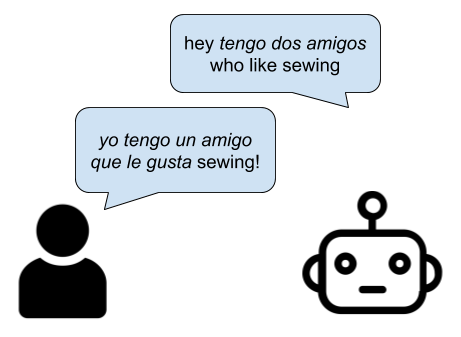
\includegraphics[width=0.5\textwidth]{img/ex_chat_1030}
	\centering
  	\caption{We build a bilingual goal-oriented system that can converse in Spanish--English CM with human users.}
    \label{fig:human-comp-chat}
\end{figure}

In order to study code-mixing in a controlled setting, we begin by modifying an existing goal-oriented dialogue framework to handle different strategies of Spanish-English CM.
We use the scenario of discussing mutual friends given a knowledge base, previously done by \citet{He2017}. 
According to this framework, both users of a system (in our case, one human and one computer) have a private table of friends with certain attributes. 
Only one friend will be the same across the two users' tables, and the goal is to find that mutual friend via collaborative discussion. 
The benefit of this symmetric collaborative dialogue is that it is task-oriented, while remaining flexible in the topics of discussion.
An example is visualized in \Fref{fig:human-comp-chat}.

To generate the text, we add modifications (visualized in green in \Fref{fig:sys-diagram}) to the original monolingual generation (in blue). 
The rule-based system generates an English string, which is passed to an Automatic Machine Translation (MT) system to receive the Spanish translation. 
The strategy transformations take the parallel English and Spanish utterances and output a CM utterance that goes to the user, and strategy condition stays fixed for the entire duration of a single dialogue.

To process the user's text, the utterance is first passed to the Machine Translation whose target language is English\footnote{This is fairly robust in converting Spanish or mixed Spanish and English into mostly English tokens}. 
The monolingual dialogue system receives the English string via the knowledge base that breaks the utterance into basic entities, all of which
% and checks if any items from the knowledge base were mentioned in order to formulate 
inform the next turn from the system.
% In our version, we update the knowledge bases and system output to be bilingual. 
% We limit our attributes to school majors, hobbies, locations, and preferred time of day. 
Named entities, as well as word pairs that have the same spelling in both English and Spanish, are omitted so that every item can be classified as clearly English or Spanish (e.g. remove `the piano' / `el piano').

% [h] means place fig "here", t=top, b=bottom
\begin{figure}
	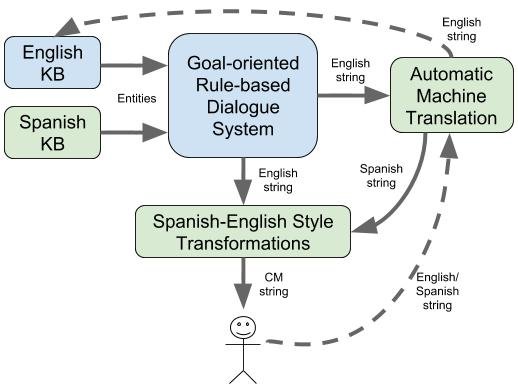
\includegraphics[width=0.5\textwidth]{img/all_system_1029}
	\centering
  	\caption{We add bilingual modules (in green) to the existing monolingual rule-based generation (in blue). The main dialogue system generates CM strings via MT and a transformer. It receives user utterances via translating into English first. \ea{TODO: increase small text size, change human to match prior fig}}
    \label{fig:sys-diagram}
\end{figure}


\section{Code-Mixing Strategies}
\label{sec:strategies}
% \yt{this is a well-written section, the only thing that should be fixed is the first paragraph, to provide a clear view of how CM strategies fit in the project. First remind about our motivation to study CM in controlled dialogues. Then say that we operationalize prior linguistic theories, site all of them. Then say that these strategies will be integrated in the bilingual collaborative dialogue setting on the bot side (point to the figure in the previous section), and that we'll analyze how people respond. then your current write-up. }
Based on prior work in CM, we chose to implement our dialogue system to produce text in three\footnote{These 3 strategies may have overlapping distribution. 
The way we calculate and report values across other corpora is by checking for Structure first, then Content. 
Social is not directly measured, and we only report 1 strategy per utterance.} specific strategies, namely Content, Structure, and Social. 
Two of these three originate from \citet{muysken2000bilingual} and have been accepted by the linguistics sub-field of CM. 
With these conditions integrated in our system, we can then analyze the different ways in which users respond to such conditions.

\subsection{Strategy: Content CM}

The first strategy inspired from \citet{muysken2000bilingual} is \textit{Insertion}, which follows the Myers-Scotton framework of a Matrix Language (ML) and an Embedded Language (EL), where the structure and grammar of the ML is maintained while inserting the EL (often single words or phrases) in certain spots \citep{myers1993common}. 
According to \citet{Joshi1982}, closed class items such as determiners, quantifiers, prepositions, possessives, auxiliaries, tense, helping verbs, etc. would remain in the ML.

This has been shown to be used more commonly when the speakers are not equally proficient in both languages \citep{Deuchar2007}. 
We define our first strategy, Content CM, to be like this insertion, such that we are keeping the grammar of English while inserting Spanish nouns, or using Spanish grammar while inserting English nouns (Example 1). 
We will refer to the former version as \textit{EN gram} and the latter as \textit{SP gram}.

\subsection{Strategy: Structure CM}

Muysken's second type of mixing is \textit{Alternation}, which is when CM adheres to constituent boundaries \citep{sankoff1981formal} and can separate topics or sentences \citep{Ardila2005}. 
This has been shown to be more prevalent in fluent or highly proficient bilinguals as a form of more stable bilingualism \citep{Deuchar2007}. 
We also include the functional head constraint in types of Structure CM generation from \citet{Belazi1994}, where switch points can occur between the lexical head and complement, (Example 2a).

We use these priors to inform our second strategy, Structure CM, where the system either begins in English for a phrase and then switches to Spanish, or begins in Spanish and then switches to English (Example 2b). 
We refer to the first as \textit{EN\textrightarrow SP} and the second as \textit{SP\textrightarrow EN}.

\subsection{Strategy: Social CM}

Lastly, since CM can occur more in casual dialogue and between people who have good rapport, we define our third strategy, Social CM, to have added discourse markers on top of either Content or Structure strategies.

Discourse markers are actively used by speakers in adding to the flow of dialogue, and they remain relatively independent of syntax or semantics \citep{schiffrin1988discourse}.
Within CM speech, these markers can be adopted as an easy form of lexical borrowing by varying levels of proficient bilinguals.
In particular, Spanish markers within English speech can be used to signify a less formal tone or to reveal Latino social identity \citep{Torres2011}.
Example 3 shows the use of \textit{you know} as the English discourse marker in a CM utterance.

Using this knowledge, we check the coverage of a set of markers\footnote{This set of common English and Spanish markers are curated from online sources and native informants.} in the Miami Bangor corpus, keeping those that occur with a frequency greater than 1\% of the tokens within CM utterances. 
We add these markers in either utterance-initial or utterance-final position.
In total we have 6 Spanish markers, 4 English markers, and 4 bilingual markers.\footnote{Additionally, we convert all numbers from numerals to text, lowercase all utterances, and sometimes add extra punctuation like ``!'' and ``...''.}
From the existing 4 strategies (2 from each of Content and Structure), there are now a total of 8 CM conditions.

\ea{is it better to have table where each strategy has a real-world example like these, and then also an example of our system's generated utterance?}

\begin{itemizesquish}
\item Example 1 -- Content (\textit{SP gram}): ``\textit{Me confirm\'o Juan que fue muy obvio, y no solamente en la} [Juan confirmed to me that it was very obvious, and not only in the] produce section, \textit{tambi\'en en el} [also in the] check-out line.'' \cite{Solorio2008}
\item Example 2a -- Structure: ``\textit{la mujer} [the woman] proud of her position'' \cite{Belazi1994}
\item Example 2b -- Structure (\textit{SP\textrightarrow EN}): ``\textit{Yo no estoy de acuerdo con eso.} [I am not sure about this.] But, anyhow, I think I will try again to get it.'' \cite{Ardila2005}
\item Example 3 -- Social: ``\textit{Yo estaba aburrecido, muri\'endome,} [I was bored, dying,] you know?'' \cite{sankoff1981formal}
\end{itemizesquish}

\subsection{Presence in other corpora}

To verify the coverage of these types of CM, we analyze their prevalence in two separate Spanish--English datasets: the Miami Bangor corpus of recorded spontaneous speech \citep{deuchar2014building} and the Twitter corpus from the 2016 Language ID shared task \citep{Molina2016}. 
Each corpus has been tagged with the language prior, \ea{continue}. 
These distributions are given in Table \ref{tab:strategy-mb-twitter} and the heuristics to automatically classify the strategies are discussed in Section \ref{ssec:eval_method}. 
We see that the most common strategy is Content CM, specifically SP gram, which follows findings from a Spanish--English corpus of blogs from \citet{Montes-Alcala2007}.

\begin{table}
\begin{center}
\begin{tabular}{l|cc}
\hline \bf Strategy & \bf Miami Bangor & \bf Twitter \\ \hline
\textit{SP gram} & 29.98\% & 45.53\% \\
\textit{EN gram} & 16.13\% & 11.33\% \\
\textit{SP\textrightarrow EN} & 16.54\% & 12.91\% \\
\textit{EN\textrightarrow SP} & 12.26\%  & 13.73\% \\
neither & 25.10\% & 19.25\% \\
\hline
\end{tabular}
\end{center}
\caption{\label{tab:strategy-mb-twitter} We verify that two of our CM strategies, Content and Structure, have a presence in two corpora.
Values are calculated on the assumption that all utterances analyzed were tagged with English and Spanish.}
\end{table}


\subsection{Research questions}
%\ea{Changed from `Hypotheses'... convert to full sentences, maybe numbered?}
Armed with a bilingual collaborative settings that operationalize 
linguistically-motivated CM strategies, 
%Given these strategies, 
we will analyze (1) how users' \emph{choice of CM} varies, 
(2) how much they \emph{entrain} to the system, 
and (3) both the \emph{extrinsic task success} as well as the \emph{perceived success} of the dialogues.
To analyze the users' choice of CM and their entrainment to our 
dialogue agent, we will explore the following research 
questions:  
\begin{itemizesquish}
\item Will certain strategies elicit more CM than others?
\item Does the presence of certain strategies follow the same CM distribution as in existing datasets (Miami/Twitter)?
\item Will the Social style of CM result in more or less entrainment than the Non-Social?
\item Will the Social style of CM result in higher task ``success''?
\item How do language proficiency, gender, and age affect user CM style?
\end{itemizesquish}


\section{Experimental Settings}
\label{sec:experiment}
In order to examine effects of different CM strategies with  human bilingual speakers, we choose to modify an existing dialogue system (\Sref{sec:dialogue-system}) and deploy it to chat with crowdworkers on two platforms.
%The methodology is described below.

\subsection{Data Collection}

We released these tasks on two crowdsourcing platforms: Amazon Mechanical Turk\footnote{https://www.mturk.com/} and Figure Eight\footnote{https://www.figure-eight.com/, originally CrowdFlower.}. 
In order to target Spanish--English bilinguals, we limited workers to be in the US,\footnote{Other countries were not included in order to limit the variance of social and cultural factors for Spanish--English CM.} and then included several ungraded Spanish proficiency test questions. 
Additionally, the introduction and instructions were purely written in Spanish to prime the user in both languages, given that English is usually the default language for tasks released in the US. 
An example of the interface shown to the user is given in Figure \ref{fig:interface}. 
In addition to the 8 CM conditions, we had 2 more monolingual conditions (Spanish and English).
For each chat, there were always 10 friends, 3 attributes, and 8 minutes on the timer for which to complete the task.

\begin{figure}
    \centering
	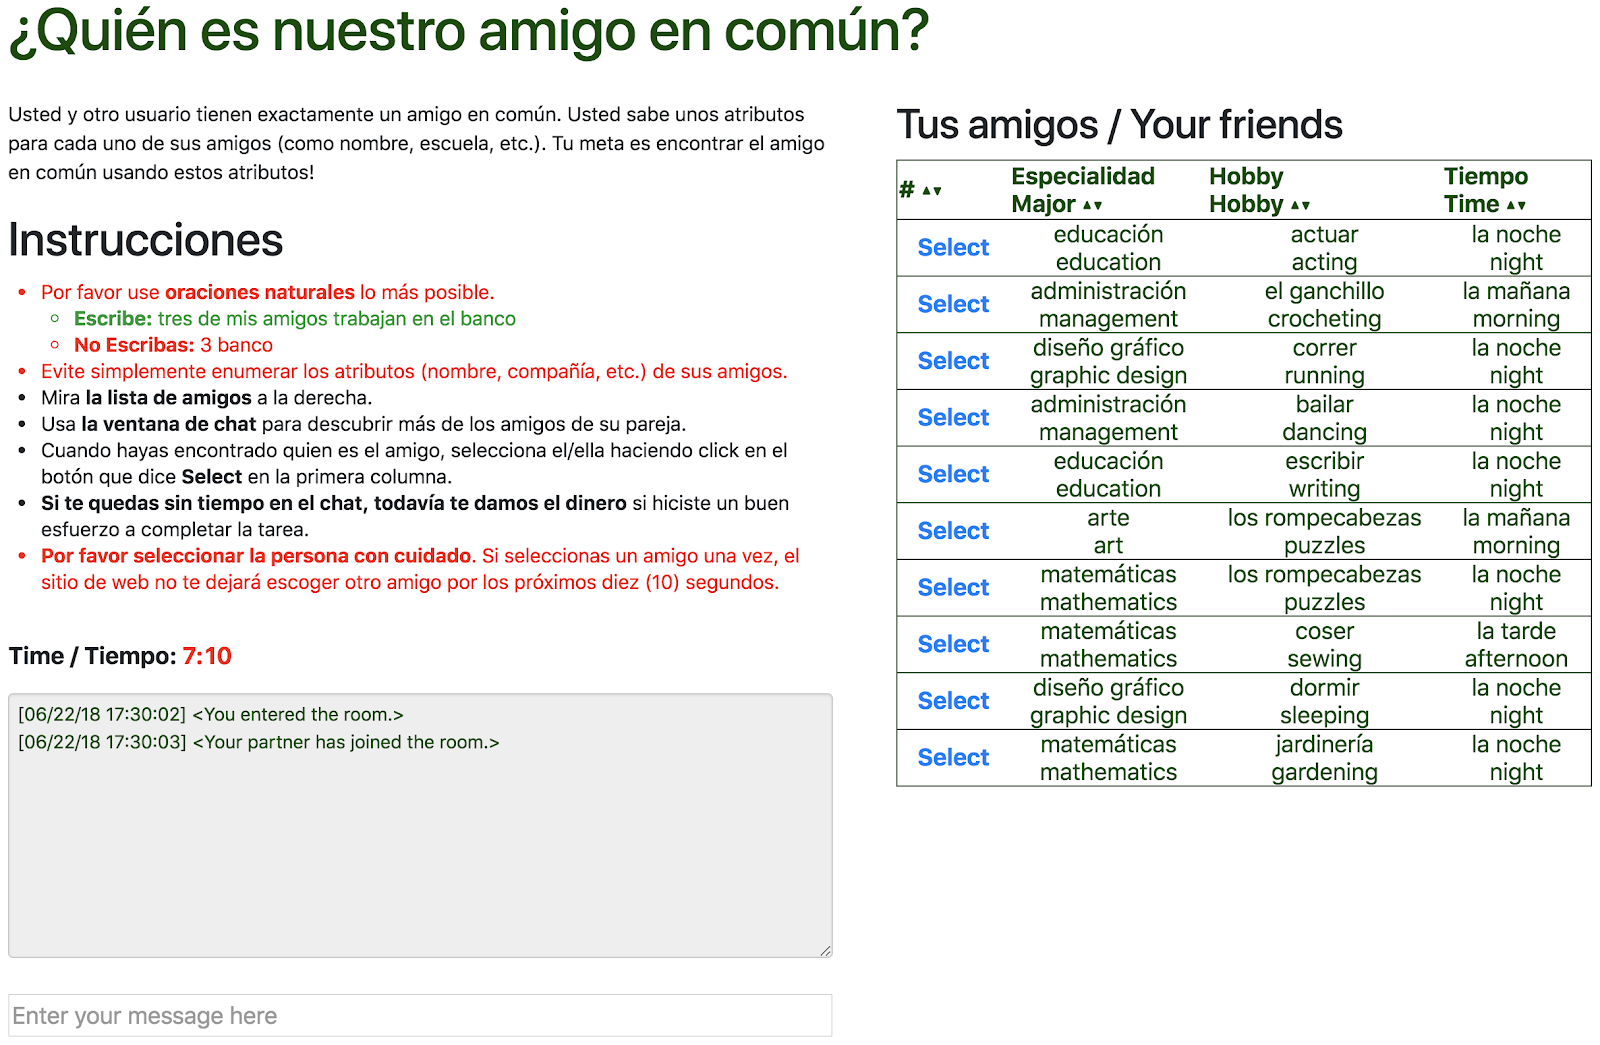
\includegraphics[width=0.5\textwidth]{img/interface_screenshot}
  	\caption{Users would see this interface when conversing with our dialogue system via text. \yt{need larger fonts; see in Yiheng's paper: https://v1.overleaf.com/18938713jhnhffvjsjnm#/71062295/}}
    \label{fig:interface}
\end{figure}

\subsection{Evaluation Methodology}
\label{ssec:eval_method}
Once the user's text data is collected, we use a few heuristics in order to analyze the amount of CM and the type of CM in a message.

\paragraph{Language Identification}
Classifying utterances on the token-level is crucial for measuring amounts and strategies of CM.

We opted for a simple look-up table style of classifying a token as English, Spanish, or neither/ambiguous. 
Each table consisted of vocabulary from the knowledge bases as well as the top 1000 most frequent words each from Spanish and English. 
Tiebreakers of entries that appeared in both languages defaulted to Spanish. 
After this automatic check, we combed through the data and manually fixed the language ID tag. 
The tokens that needed fixing typically fell into the categories of spelling typos, homographs that appear in both languages (e.g. \textit{a} and \textit{me}), and inflections of common verbs (e.g. \textit{estudie/estudiado}).

\paragraph{Strategy Classification}
We propose a novel method to classify CM utterances into one of four strategies (2 types for each of Content and Structure).\footnote{Note this is the same metric used to calculate strategies in the Miami Bangor and Twitter corpora.}

An utterance would be a Structure switch from Lang\textsubscript{A} to Lang\textsubscript{B} if there is at least one Lang\textsubscript{A} function word followed by at least one Lang\textsubscript{B} function word.
If the utterance is not classified as Structure, it would be tested for Content next. 
We have defined Content to occur where the matrix language should have more function words than the embedded language, and the embedded language has at least one content word.\footnote{Content is determined by [`NOUN', `ADJ', `VERB', `PROPN'] from Myers-Scotton's framework. These POS tags were generated by English and Spanish POS tags from Spacy, available at https://spacy.io/.}
\ea{Do I need to show the ``goodness'' of this classification technique?}


\section{Results}
\label{sec:results}

\ea{overview of section}

\subsection{Collected Dialogues}
We report general statistics of our collected dialogues in Table \ref{tab:overview-stats}.

\begin{table}[]
\centering
\begin{tabular}{ll}  % l
                                %  & \textbf{Ours} & \textbf{\citet{He2017}} \\ 
\hline
\# dialogues                     & 587    \\ %  & 11157      \\
\% `successful' dialogues        & 63\%   \\ %  & 81\%       \\
avg \# user utterances           & 8.09   \\ %  & 11.41      \\
avg \# tokens / utterance        & 6.13   \\ %  & 5.08       \\
% following # is for entire turk task, not simply time w/ chatbot
% avg time per task (min)          & 10.1    \\ %  & 91.18      \\ 
EN vocab size                    & 571    \\ %  & 5325       \\
SP vocab size                    &  846    \\ %  & --         \\
\% EN utterances                 & 16\%   \\ %   &  --      \\
\% SP utterances                 & 44\%   \\ %   &  --      \\
\% CM utterances                 & 39\%   \\ %   &  --      \\
\% dialogues w/ CM               & 74\% \\ %  & -- \\ 
\hline
\end{tabular}
\caption{Our corpus has a strong presence of CM and uses language \red{richly}.}
\label{tab:overview-stats}
\end{table}
% Old caption: General statistics of our dataset. Success here is the extrinsic task success of finding the mutual friend or not.

A total of 737 dialogues were collected, but 587 remain for analysis after removing 112 which contained no text from users\footnote{Not typing back to the dialogue system is allowed, and users can just click on different friends until they achieve the extrinsic goal.} and an additional 38 of those who did not take the survey.

Many workers took more than one task, so from the pool of 587 valid chats, there were 322 unique workers across the two platforms. 
From the self-reported survey, 61\% of the workers were male, the mean age was 31, and the most frequently reported countries of origin were USA, Venezuela, and Mexico.

Examples of conversations gathered of our dialogue system with crowdsourced bilinguals are given in Table \ref{tab:example-dialogues}.
It is interesting to find that in the \textit{SP\textrightarrow EN} Structure condition, even when the system uses the Spanish word \textit{contabilidad}, the user chooses to emulate the strategy instead of echoing that lexical item.
They say the equivalent meaning in English, which is \textit{accounting}.
In the same way, when the \textit{SP\textrightarrow EN} system discusses \textit{dancing}, the user replies with the Spanish equivalent, \textit{bailar}, thus adhering to the strategy.

\begin{table*}[t]
\centering
\begin{tabularx}{\linewidth}{sb|sb}
% \toprule
\hline
\multicolumn{2}{c}{\bf\textit{EN\textrightarrow SP}} & \multicolumn{2}{c}{\bf\textit{SP gram}} \\  
\hline
S: & I have 2 friends \textit{que estudiaron la contabilidad} [that studied accounting] & S: & \textit{?`Tiene} [Do you have] friends \textit{que trabajen en el} [who work at the] theater \textit{o un} [or a] friend \textit{que trabaje en la} [that works at the] jewelry store ?
\\

H: & \textit{yo tambien} [me too]. one that studies accounting \textit{trabaja en el concesionario de coches y el otro en la oficina} [works at the car dealership and the other in the office] & H: & \textit{si. la del} [yes. the one from] jewelry store \textit{le gusta dormir} [likes to sleep]
\\
S: & Do you have any friend who likes dancing \textit{o amigos a los que les guste hornear} [or friends who like to bake]? & S: & \textit{tengo} [I have] 1 friend \textit{que le gusta} [who likes] acting, 1 friend \textit{que trabaja en el} [who works at the] zoo
\\
H: & \textit{nadie le gusta bailar} [no one likes to dance]. one likes baking--\textit{el/ella estudia fisica} [he/she studies physics] & H: & \textit{la del teatro le gusta} [the one from the theater likes] photography
 \\
% \bottomrule
\hline

% \textit{EN\textrightarrow SP +SOC}
% S: & hey do you have any friends \textit{trabajando en el banco} [working at the bank]?
% H: & no \textit{mi} [my] exgirlfried \textit{era cajera en un} [was a cashier at a] bank \textit{pero ya no hablamos} [but we don't talk anymore]
% \textit{SP gram +SOC}
% H: & \textit{estudian} [do they study] education?
% S: & yeah \textit{tengo un} [I have a] friend \textit{que estudi\'o} [who studied] education
% H: & have a friend \textit{que} [that] likes \textit{leer} [to read]?
% S: & ah ok \textit{yo tengo} [I have]!

\multicolumn{2}{c}{\textbf{\textit{SP\textrightarrow EN +SOC}}} & \multicolumn{2}{c}{\textbf{\textit{EN gram +SOC}}} \\  
% \midrule
\hline
S: & \textit{tengo un amigo} [I have a friend] who studied english.. \textit{y t\'u} [and you]? & S: & do you have any \textit{amigos} [friends] who studied \textit{derecho} [law] ?
\\
H: & \textit{no tengo... solo tengo un amigo que estudio} [I don't have... I only have a friend that studied] linguistics & H: & no i don't
\\
S: & hey \textit{tengo dos amigos} [I have two friends] who like sewin & H: & \textit{tienes un amigo a quien le gusta cocinar} [do you have a friend who likes to cook]?
\\
H: & \textit{yo tengo un amigo que le gusta} [I hve a friend that likes] sewing! & S: & nah i have no \textit{amigo} [friend] who likes \textit{cocinar} [to cook]..
\\

%   \bottomrule
\hline
\end{tabularx}
\caption{\label{tab:example-dialogues} Examples of human (H) interactions with 4 different dialogue systems (S).}
\end{table*}

\section{Analysis}
\label{sec:analysis}

% \ea{overview of section.. Interplay between amount of CM, entrainment, levels of success, social conditions, and other user factors}

Now we examine in finer detail the subtleties of how users code-mixed under different conditions, whether user or system strategies contributed to dialogue success, and the effects of demographic factors.

\subsection{Types of User Code-Mixing}
% \ea{use more excited language, frame how cool this is!}
From the results of our corpus, we find that a high majority of dialogues contain CM from the user (Table \ref{tab:overview-stats}).
The questions now are how much CM did users do, how did they do it, and how much did the system strategy conditions factor into response style?

We first analyze the amount or presence of CM by calculating metrics defined in \citet{guzman2017metrics}. 
The Multilingual-index (M-idx) reflects the balance of tokens in each language, where 0 = monolingual and 1 = equal \# of tokens per language. 
The Integration-index (I-idx) is the probability of switching languages between any two tokens, where 0 = a parallel corpus and 1 = a perfectly interleaved corpus.\footnote{To calculate I-idx in a given dialogue, all utterances are collapsed in order and switch-points can occur across utterance boundaries.}
Higher values of both indices imply a higher quantity of mixing. 
From Figure \ref{fig:general_tbl}, we see \textit{EN gram +SOC} and Structure conditions resulting in higher M-indices than average. 
Most notably, \textit{SP gram} results in the lowest M-idx and I-idx. 
\textit{SP gram} had more monolingual Spanish text from users than any other condition, which likely contributed to the lower indices, and this could have resulted from the experimental setup priming users to be in Spanish mode.
Conversely, \textit{EN gram} maintains a markedly higher I-idx. 

From the numbers in the general information found in Figure \ref{fig:general_tbl}, we can recommend that if future CM dialogue systems desire to be efficient in number of turns, the EN gram strategy is useful, but if they want to chat for longer, EN gram +SOC or SP\textrightarrow EN +SOC could yield more turns. \ea{continue}

\begin{figure*}[t]
    
	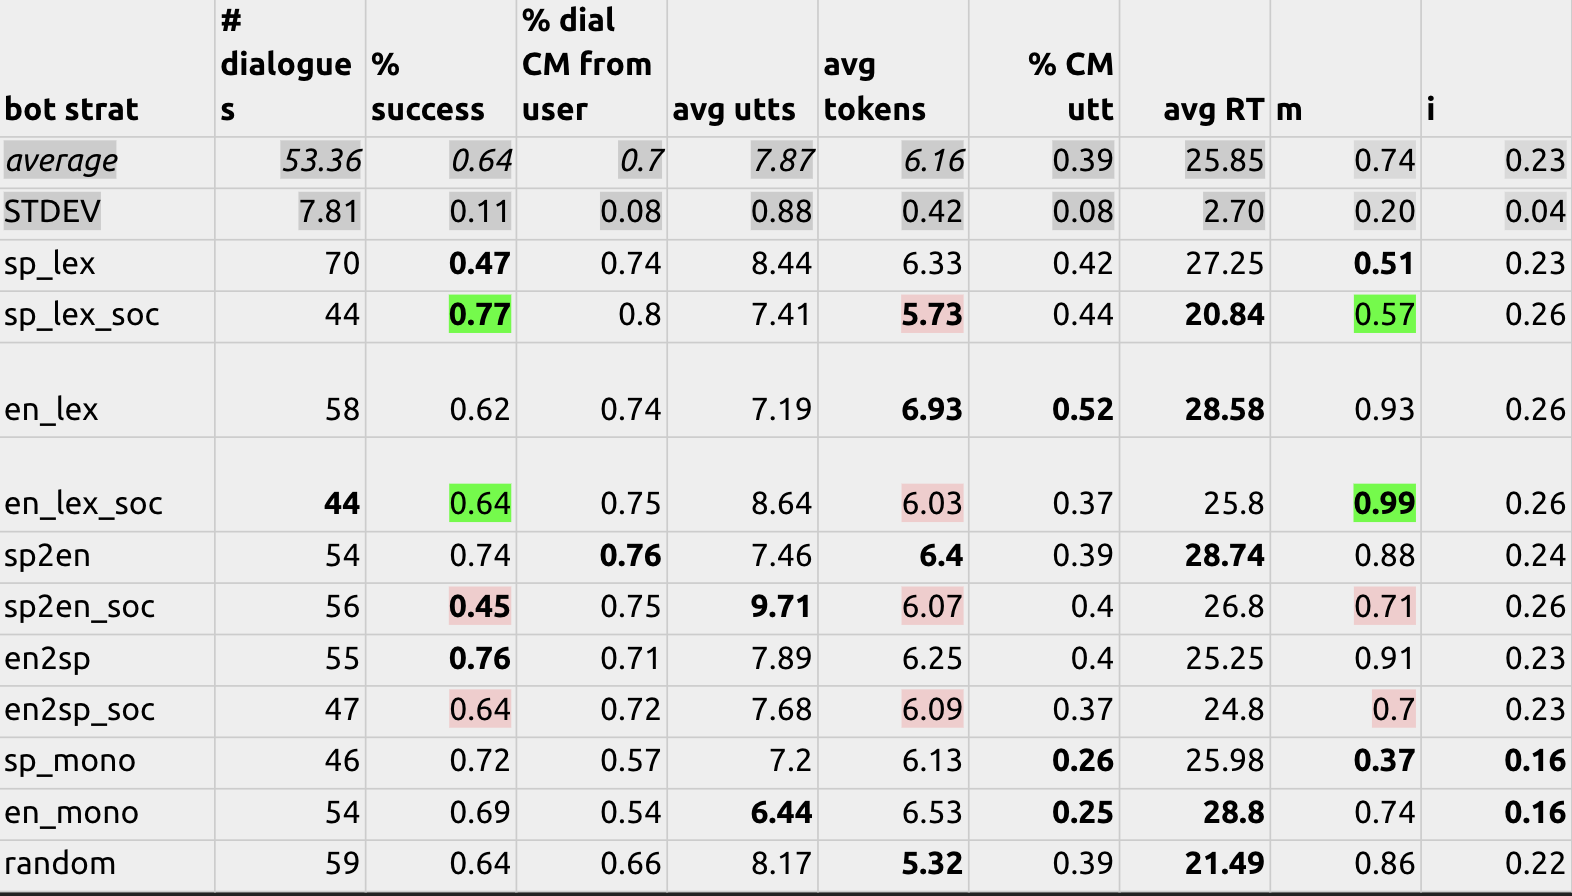
\includegraphics[width=\textwidth]{img/0927_tbl_general}
	\centering
  	\caption{\red{Change to LaTeX table.} Statistics including mean and standard deviation (SD), for each system condition. Items further than 1 SD away from the mean are in \textbf{bold}. \ea{split into 2 tables: general info and CM info}}
    \label{fig:general_tbl}
\end{figure*}

% \ea{Maybe TODO: discuss \%s of presence of CM/Spa/Eng utterances
% Compare distribution with Miami/Twitter}

% \ea{Maybe TODO: within group effects of conditions, vs random baseline.}

\subsubsection{Entrainment}

We now try to answer if the user entrained to the system -- whether they copied the amount of CM or the CM strategy of the system.

With respect to quantity of CM, we would predict Structure-based CM to have a lower I-idx since switches are likely to be more periodic and less frequent.
Yet while the Structure strategies from the system produced utterances with lower I-indices, the same pattern is not found significantly from the users' responses. 
Users seem to have a stable I-idx across all CM conditions, and thus they are not entraining to the I-idx. 
As for the M-idx, the Structure conditions produce utterances that are nearly at 1.0, which is higher than the Content conditions. 
However, we do not see this trend in the users -- the M-idx is low for SP gram, middle in Structure conditions, and highest in EN gram.
Presumably since \textit{SP gram} is the strongest strategy to be repeated back, the quantity of English tokens would be much less (thus a lower M-idx). 

\begin{figure}
	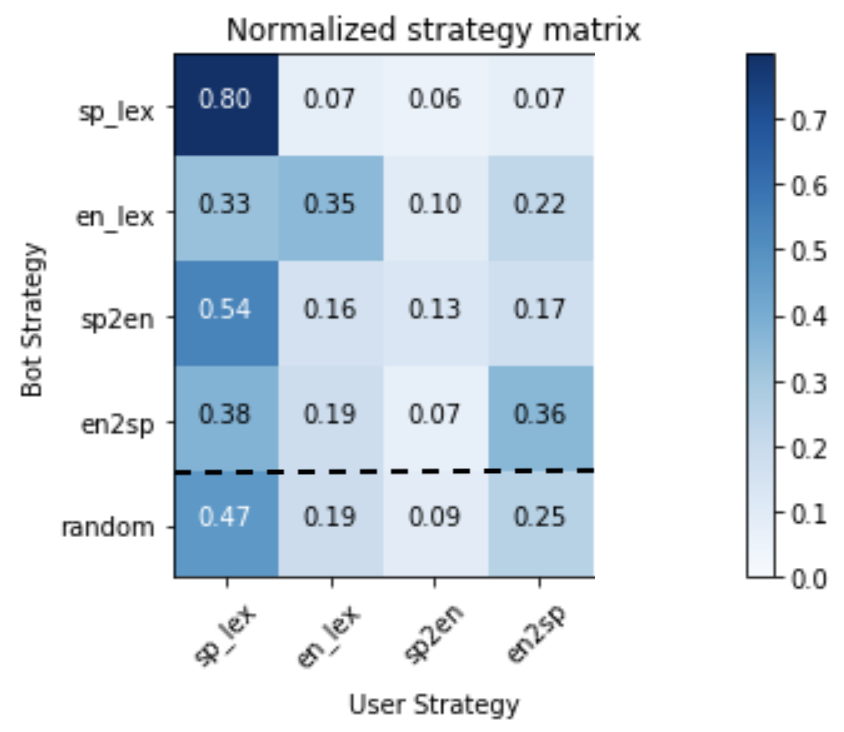
\includegraphics[width=0.5\textwidth]{img/0924_entrain}
	\centering
  	\caption{\red{Update Matrix.} We find entrainment in our data. Given each system strategy condition (per row), we display the normalized distribution of which strategies the users used (only accounting for utterances that are code-mixed). A darker line along the diagonal indicates complete entrainment, and the random system strategy at the bottom is shown for comparison.}
    \label{fig:entrain_matrix}
\end{figure}

At the strategy level, from the metrics we defined in Section \ref{ssec:eval_method} to classify a CM utterance, we see the presence of entrainment between system strategy (condition) and user strategy. 
From the strategy matrix in Figure \ref{fig:entrain_matrix}, perfect entrainment  (where all the users' CM utterances use the same fixed system strategy) would be shown with a normalized value of 1.0 along the diagonal. 
We compare values across CM conditions (without examining +SOC for now) to the random baseline, which ideally reveals the natural distribution of user strategy without a pre-fixed condition.\footnote{Reassuringly, the percentages in this random condition are similar to the distribution of the Miami Bangor and Twitter corpora from Table \ref{tab:strategy-mb-twitter}.}
Sure enough, the values on the diagonal are greater than in the random condition.

Upon a closer look, \textit{SP\textrightarrow EN} is the least commonly used strategy from users, as well as the weakest strategy to be entrained. 
In that system condition, more of its user utterances are being classified as \textit{SP gram}, which is at least  consistent with the matrix language that the system begins with.
For the conditions where English is the main (or starting) matrix language, \textit{SP gram} occurs less, while other English-based CM strategies are used more often. 
We also see more sensitivity to the specific English strategy because more utterances are classified as \textit{EN gram} in \textit{EN gram} conditions or \textit{EN\textrightarrow SP} in \textit{EN\textrightarrow SP} conditions.
Overall, \textit{SP gram} is the most popular strategy used---it is best reflected in the \textit{SP gram} condition, but still keeps strong presence in the other conditions as well.


\subsection{Dialogue Success}

We define two types of Success in the dialogues:

\begin{enumerate}
\item Extrinsic success (the binary extrinsic goal of finding the mutual friend in the given 8 minutes).
\item Perceived success (self-reported measures on scales of agreement from 1-5, e.g. \textit{I understood the task perfectly}, or \textit{My task partner texts like someone I know}).
\end{enumerate}

Using Pearson's $r$, we examine if the quantity of CM or the level of entrainment have correlations with both types of success.
All results are considered significant with $r^2$ > 0.2.

While M-idx and I-idx did not correlate with the binary extrinsic goal, M-idx negatively correlated with number of turns in the dialogue ($p$ < .001).
This means that less presence of tokens in both languages from the user resulted in a quicker chat.
A possible reason is that quicker chats means the user succeeded in finding the friend early, yet there was no significant negative effect of extrinsic goal; instead, intuitively there could be less chance for mixing when the user speaks across fewer turns.
As for perceived success, when users reported that they understood the task better, M-idx and I-idx were higher ($p$ < .001).
It is likely that the task primed users to code-mix.\footnote{The instructions encourage users to use English, Spanish, or a mixture of the two. The title of the crowdsourced task is also called \textit{``Charlemos en Spanglish!''}, meaning ``Let's chat in Spanglish!''}

We quantify the entrainment score within one dialogue to be a ratio of the number of user utterances that copy the given a system strategy, over the total number of CM user utterances. 
Ultimately, we do not find significant correlations (of r\textsuperscript{2} > 0) between this entrainment score and any type of success metric.
 This implies that the different system strategies of CM do not affect the perception of the user, making it more seamless to use different strategies interchangeably. 
Having some opacity in the link between strategy and task success could allow future CM dialogue systems to be diverse in strategy, which gives future work a chance to find more optimal and nuanced ways to incorporate CM into these intelligent agents.

\ea{Maybe TODO: how does the distribution of our entrainment values compare to those from MIAMI?}

\subsection{Effect of Social CM}
The third dimension of CM, namely the added social/informal strategy, has a number of interesting effects that interplay with Content and Structure conditions.
For all four conditions, it reduced the average number of tokens in the reply from the user, which could be a result of users being more casual with the dialogue system.
We now examine this factor with three of the measures discussed previously.

Firstly, there are interesting effects on the users' amount of CM.
When the social discourse markers are added, the M-idx increases for both Content strategies while it decreases for both Structure strategies. 
\ea{When I look at examples qualitatively, I can't see why this happens...}
The I-idx slightly increases for all strategies except for \textit{EN gram}.

Secondly, adding social and informal styles does not have a significant effect on any type of dialogue success.
\ea{++ ?}

Lastly, for most strategies except for \textit{EN gram}, a more social system results in less entrainment (lower normalized scores along the diagonal if visualized in a table similar to Figure \ref{fig:entrain_matrix}).
We find that the users are generally using more \textit{SP gram} in their chat.
The \textit{EN gram} condition is the exception, where {EN gram +SOC} led to users emulating \textit{EN gram} more.

\ea{TODO: calculate users' amount of socialness (presence of discourse markers)}

\subsection{Effect of User Type}

We examine the effect of different user attributes, namely language proficiency and other demographic information such as age, gender, and country. 
\ea{Any confounding factors? platform (MTurk vs Figure 8)?}

\paragraph{Language Proficiency}
We measure proficiency from the self-reported scores of users' own English and Spanish ability, on a 5-point scale.
% several self-reported metrics, which include a 5-point scale of English and Spanish ability, age one began to learn each of the two languages, and scores from a 3-question quiz\footnote{We passed everyone who took the quiz, and given the location constraint was the US, we did not release an English proficiency quiz.} on Spanish grammar that we created.
Our findings support the hypothesis from \citet{Deuchar2007} in that more proficient bilinguals (balanced in both languages) use Structure strategy more often than asymmetrical bilinguals. 
We examine this by binning the groups into three categories from the self-reported language ability metric: highly proficient in both (high ENG and high SPA, 207 users), dominant English (high ENG and low SPA, 77 users), and dominant Spanish (high SPA and low ENG, 29 users). 
Compared to the aggregate report of user CM, dominant English speakers use \textit{EN gram} more heavily, while dominant Spanish speakers use \textit{SP gram} more heavily.
Structure CM occurs in those two groups but is more present in the balanced bilingual group.
Although the quantity of chats for the asymmetrical bilinguals is low, our findings support the original hypothesis.

For the dominant English speakers, a higher M-idx correlated with them better agreeing on statements such as ``My task partner was very cooperative'' ($p$ < .05).
When these users entrained more to the system's CM strategy, the number of turns in the dialogue also increased ($p$ < .05). 
Also, extrinsic task success for them were low on the monolingual Spanish condition, while all CM conditions (except \textit{SP\textrightarrow EN +SOC}) boosted task success.
These findings together show that the dialogue experience overall improves for less-balanced bilinguals when the system uses CM.
This supports a line of pedagogy that would incorporate CM in second language instruction.
\ea{not enough dialogues, only 2-6 per condition, to make conclusions for dominant Spanish speakers.}

\paragraph{Demographic Factors}
Reported gender\footnote{``Other'' gender was set aside for this analysis.} yielded strong findings on the effect of social conditions.
% , women on average had a slightly higher M-idx (by .06), yet an identical I-idx.
With the social discourse markers, women consistently had higher percentages of CM utterances than men (a difference of 4-11\% for each condition).
Yet without social strategy, men had equal or higher percentages of CM utterances than women (an exception being \textit{EN gram}). 
This same pattern can be seen in \% dialogues containing CM where women have higher values in social condition while men are the reverse, but the exception for men is that for \textit{SP gram}, women still had more CM dialogues than men (though less strongly than in \textit{SP gram +SOC}.
Again this holds for number of utterances per dialogue. 
With added social strategy, women had an 1-3 extra utterances while without social strategy the men had more utterances (again with one exception that in \textit{SP\textrightarrow EN}, women still had more utterances than men, but less strongly than in \textit{SP\textrightarrow EN +SOC}).
In summary, women responded to social conditions such that they had longer dialogues and more CM, which proved to be an opposite effect for men.
\ea{Do I need to support previous stats with \#s in a table?}

Lastly, reported age also affects user styles.
We use a threshold of 35 to split users into younger and older age categories, with the latter group yielding 22\% of all dialogues.
Compared to older users, younger users on average achieved extrinsic success 12\% more often, used more CM, and had longer conversations (more utterances, but slightly less tokens per utterance).

% \paragraph{User Response Style}
% \ea{Would this sub-section be interesting? I haven't calculated these things yet.}
% What happens when user uses certain strategies? When user uses short vs long utterances? 
% More or less turns? 
% More punctuation and capitalizing text (indicating formal style)? 
% Amount of CM and CM strategy?

\subsection{User Feedback}
Users of this study overall had positive impressions of their dialogue experience.
They mostly agreed to the statement \textit{``If technology (like Siri or Alexa) progressed to allow me to use Spanglish, I could see myself using both languages with it''}, and this is an encouraging sign for future systems that want to incorporate Spanish--English CM in their dialogue.
%  (aggregate 4.14/5.0, meaning ``Mostly Agree'')

Some common critique we received was similar to this user's experience: ``my partner was all over the place. It was hard to keep up with all their \textit{preguntas} [questions]. I don't think we ever found our \textit{amigo en comun} [mutual friend].''
Given that our system is rule-based, it could often dominate the conversation and lead users down specific dialogue patterns, but this is a common effect known about rule-based systems \ea{CITE}.
There is room for future work to incorporate bilingual code-mixing into more advanced dialogue systems like the knowledge graph-based system from \citet{He2017}.

Another valuable comment validated several of our goals.
A user who had the \textit{EN gram +SOC} condition said, ``in my experience speaking with other bilingual friends the switching is usually either half of the sentence or alternating sentences... Rarely do I just use one word in the other language unless it's pretty specific to that language... But I found myself doing it along with the robot!''
He acknowledged that he would naturally use a more alternating, Structure strategy of CM, but \red{admits} to entraining to the system who uses a Content strategy.



\section{Related Work}
\label{sec:related-work}

We provide a brief overview of previous works in the domains of code-switching (CS) and dialogue.

% From fields of NLP and Linguistics,

Attempts have been made to integrate CM into NLP areas such as Part-of-Speech tagging \citep{Solorio2008,soto2018joint}, Language Identification \citep{soto2018joint,Rijhwani2017}, Named Entity Recognition \citep{aguilar2018named}, Language Modeling \citep{chandu2018language}, Automatic Speech Recognition (ASR) \citep{yilmaz2018building}, and Speech Synthesis \citep{Rallabandi2017}.
There also has been a push to generate CM datasets synthetically to improve CM language modeling \citep{pratapa2018language}, or manually crowdsource CM utterances towards CM Question--Answering and dialogue systems \citep{chandu2018code,banerjee2018dataset}.
% Code-mixed corpora are emerging, such as the code-mixed DSTC2 restaurant reservation dataset where crowdworkers manually translated from English into various Indian Englishes---this dataset was built with the intention of developing future goal-oriented dialogue systems \citep{banerjee2018dataset}.
% Our corpus differs in that one partner is an agent while the other is responding to this specific scenario in real-time.

% Another ASR paper from 2017: Amazouz2017, sivasankaran2018phone
% predict switch points from one language into another
% \citet{Fricke2016} also discovered the importance of acoustic cues in determining when users will code-switch.
% Pratapa et al. (2018) used syntactic linguistic theory to generate synthetic code-switched data, which could aid in CM language models ().

Various other research has centered around understanding when and why people code-switch.
Linguistically-driven methods have found that cognates and acoustic cues allow for more fluid switching between the languages \citep{kootstra2012priming,Fricke2016}.

When pertaining to a dialogue setting, CM has been found to fulfill different goals of speakers. \citet{Solorio2008} discussed how sociopragmatic factors, such as the topic being discussed and the rapport between the speakers, could influence the style of CM.
In support of this, \citet{Yoder2017} showed that the use of code-mixed English marked positive social influence in a study of Arabic Wikipedia editor talk pages.
Additinoally, choosing to use one language over another can be a pragmatic way to mark sentiment, as \citet{rudra2016understanding} found in Hindi--English Twitter data.
% and found that Hindi was more popularly used for expressing negative sentiment.

Entrainment in bilingual human--human dialogues has been recorded since \citet{giles1973towards} where French--English speakers would choose their language according to their audience.
More recently in entrainment of CM, \citet{soto2018role} showed a convergence in the quantity of CM between speakers over the course of long conversations in the Miami Bangor data.
The presence of CM can affect the utterance following it \citep{fricke2016primed}.


\section{Conclusion}
\label{sec:conclusion}

% sentences taken from intro. MODIFY:
% In this study, we controllably analyze the different strategies in which people may code-mix in dialogues, in order to pragmatically and linguistically learn what makes for successful CM interactions between humans and computers. 
% A successful human--computer dialogue can be determined in ways such as achievement of an explicit goal, or naturalness of a conversation that indicates better rapport.
% We incorporate linguistically-motivated strategies of CM into a rule-based, goal-oriented dialogue system, and analyze the amount of CM, strategy type, and amount of entrainment that a bilingual user has with respect to the system strategy conditions.
% With these measures, we present analyses of each strategy's effect on the amount of elicited CM and amount of entrainment with respect to dialogue success.


\red{In our novel Spanish--English dialogue framework, we have generated CM utterances that users generally accepted and responded back in various forms of CM.
We show that it is useful to break down CM dialogue into different strategies, as was a research suggestion from \citep{bullock2018should}, and we implement \red{novel} metrics to calculate and generate these strategies in Spanish--English.
Users favor the \textit{SP gram} strategy, but are adaptable to other strategies when fixed as the system condition.
They also differ in strategy use depending on bilingual language proficiency.
Adding discourse markers to make the system more ``social'' produced outcomes from users such as shorter utterances, less entrainment, and strategy-specific and gender-specific patterns in quantity of CM.
Task success and perceived dialogue success were not hugely affected by CM strategy, but some effects were found from reported age of users.}
\ea{previous sentences used in Intro. switch it up for this conclusion}

% effectively learn about the bilingual mind and the linguistic and social triggers of code-mixing

Clear future work involves having the system use different CM strategies dynamically within a single conversation. 
Then we could move towards studying and implementing a CM system that entrains to the user.
% , since systems accommodating to a user's style has been shown to provide better user experience and task completion \ea{CITE}.
However, knowing which CM strategies are more entrainable than others could help systems to better parse and predict user utterances with a more informed language model, similar to a method where ASR systems that lexically entrain users can lower ASR error rates \citep{levitan2013entrainment}. 
% Topics of dialogue should also expand beyond the task of discussing hypothetical friends with a limited number of attributes.

With this data, follow-up analysis can be done on the types of switch points, investigating for example the simplicity or frequency of the word that is switched or the nature of being a cognate \citep{soto2018role}, or even the cognitive accessibility of switch points words from users' mental lexicon.

Future work can also be done on other language pairs such as Hindi--English, with beneficial analysis on how linguistically and functionally similar or different the CM strategy usage would be, as compared to Spanish--English.

% Other applications include educational purposes.
% Labutov \& Lipson (2014)
% Renduchintala+ (2016)
% ``Macaronic'' interfaces for L2 learning

We can usher in an era of bilingual dialogue systems that brings human--computer interactions to a more personalized space.
\ea{++ ?}

% \section{Appendices} 
% Anything to move here?


\iftaclfinal

\section{Acknowledgments}
Thank God for funding. Include some nice words to nice people.
\else
\fi

\bibliography{tacl}
\bibliographystyle{acl_natbib}

\end{document}